\documentclass[spanish]{beamer}
\usepackage[utf8]{inputenc}
\usepackage{float}
\usepackage{beamerthemesplit}
\usepackage{latexsym}
\usepackage[T1]{fontenc}
\usepackage{amsmath}
\usepackage{hyperref}
\usepackage{graphicx}
\usepackage{babel,blindtext}
\usepackage{amsfonts}
\usepackage[round]{natbib}
\bibliographystyle{chicago}
\usepackage{subcaption} 


\decimalpoint

\usetheme{Antibes}%este es el templete que se usa a lo largo de la presentacion
%themes
%   default
%   Boadilla
%   Madrid
%   Pittsburgh
%   Copenhagen
%   Warsaw
%   Singapore
%   Malmoe
\newcommand\Fontvi{\fontsize{6}{7.2}\selectfont}
\mode<presentation>%tipo de 
\begin{document}

%%%%%%%%%%%%%%%%%%%%%%%%%%%%%%%%%%%%%%%%%%%%%%%%%%%%%%%%%%%%%%%%%%%%%%%%%%%%%%%%%%%%%%%%%%%%%%%%%%%%%%%%%%%%%
\title{Markov Chains}
\author{Gamaliel Moreno Chávez}
\institute{MCPI}
\date{Ago-Dic\\ 2020}%para que ponga la fecha de hoy 

\frame{\titlepage}
%%%%%%%%%%%%%%%%%%%%%%%%%%%%%%%%%%%%%%%%%%%%%%%%%%%%%%%%%%%%%%%%%%%%%%%%%%%%%%%%%%%%%%%%%%%%%%%%%%%%%%%%%%%%%
%%%%%%%%%%%%%%%%%%%%%%%%%%%%%%%%%%%%%%%%%%%%%%%%%%%%%%%%%%%%%%%%%%%%%%%%%%%%%%%%%%%%%%%%%%%%%%%%%%%%%%%%%%%%%%%%%%%%%%%%%%%%%%%%%%%%%%%%%%%%%%%%%%%%%%%%%%%%%%%%%%%%%%%%%%%%%%%%%%%%%%%%%%%%%%%%%%%%%%%%%%%%%%%%%%%%%%%%%%
%%%%%%%%%%%%%%%%%%%%%%%%%%%%%%%%%%%%%%%%%%%%%%%%%%%%%%%%%%%%%%%%%%%%%%%%%%%%%%%%%%%%%%%%%%%%%%%%%%%%%%%%%%%%%%%%%%%%%%%%%%%%%%%%%%%%%%%%%%%%%%%%%%%%%%%%%%%%%%%%%%%%%%%%%%%%%%%%%%%%%%%%%%%%%%%%%%%%%%%%%%%%%%%%%%%%%%%%%%

\begin{frame}
\frametitle{Introducción}
\begin{center}
{\huge ¿cuál es la característica principal de un procesos Markoviano?}
\end{center}

 
\end{frame}

%%%%%%%%%%%%%%%%%%%%%%%%%%%%%%%%%%%%%%%%%%%%%%%%%%%%%%%%%%%%%%%%%%%%%%%%%%%%%%%%%%%%%%%%%%%%%%%%%%%%%%%%%%%%%
\begin{frame}
\frametitle{Estados y transiciones} 
Cadenas de Markov
\begin{itemize}
\item Secuencia de paso o intentos discretos numerados por $n=0,1,2,\ldots$
\item El resultado de n-th intento es la variable aleatoria $X_{n}$
\item $X_{0}$ es la posición inicial de proceso. Esta variable aleatoria puede tomar valores $i=1,2,\ldots, m$ 
\item El resultado actual es llamado estado del sistema y se donota como $E_{i} (i=1,2,\ldots, m)$
\end{itemize}
\footnotetext[1]{La caminata aleatoria es un caso especial de un proceso más general, el de Markov .}
´\end{frame}
%%%%%%%%%%%%%%%%%%%%%%%%%%%%%%%%%%%%%%%%%%%%%%%%%%%%%%%%%%%%%%%%%%%%%%%%%%%%%%%%%%%%%%%%%%%%%%%%%%%%%%%%%%%%%
\begin{frame}
\frametitle{Estados y transiciones}
Cadenas de Markov

Si la v.a.s $X_{n-1} = i$ y $X_{n} = j$, entonces el sistema ha realizado un transición $E_{i} \rightarrow E_{j} $, esto es, una transición del estado $E_{i}$ al estado $E_{j}$ en el intento n-th.

Notese que $i$ puede ser igual que $j$, las transiciones al mismo estado son posibles.
La asignación de potabilidades a las transiciones de $E_{i} \rightarrow E_{j}$ es conocida como cadena

\end{frame}
%%%%%%%%%%%%%%%%%%%%%%%%%%%%%%%%%%%%%%%%%%%%%%%%%%%%%%%%%%%%%%%%%%%%%%%%%%%%%%%%%%%%%%%%%%%%%%%%%%%%%%%%%%%%%
\begin{frame}
\frametitle{Cadenas de Markov}
Las cadenas de Markov tiene la propiedad de que la probabilidad de que $X_{n}=j$ depende solamente del estado previo del sistema.  Formalmente, esto significa que no necesitamos más información en cada paso que, para cada i y j.


\begin{multline*}
P\lbrace X_{n} = j\vert X_{n-1} = i\rbrace = P\lbrace X_{n} = j\vert X_{n-1} = i, X_{n-1} = K_{n-1},\\ X_{n-2} =  K_{n-2}, \ldots X_{1} = K_{1} \rbrace
\end{multline*}
lo que  significa que la probabilidad $X_{n} = j$ dado $X_{n-1} = i$: es independiente de los valores $X_{n-2} , X_{n-3},  \ldots, X_{1}$. 
\end{frame}

%%%%%%%%%%%%%%%%%%%%%%%%%%%%%%%%%%%%%%%%%%%%%%%%%%%%%%%%%%%%%%%%%%%%%%%%%%%%%%%%%%%%%%%%%%%%%%%%%%%%%%%%%%%%%
\begin{frame}
\frametitle{Cadenas de Markov}
Conceptos básicos
\begin{itemize}
\item Probabilidad de transición 
\item Probabilidad estacionaria o absoluta
\item Probabilidad de transición en $n$ pasos
\end{itemize}
\end{frame}


%%%%%%%%%%%%%%%%%%%%%%%%%%%%%%%%%%%%%%%%%%%%%%%%%%%%%%%%%%%%%%%%%%%%%%%%%%%%%%%%%%%%%%%%%%%%%%%%%%%%%%%%%%%%%
\begin{frame}
\frametitle{Probabilidades de transición}
Para una cadena de Markov finita con $m$ estados $E_{1}, E_{2} ,\ldots, E_{m},$  tenemos 
\begin{equation*}
p_{ij} = P\lbrace X_{n} = j \vert X_{n-1} = i\rbrace,
\end{equation*}

donde $i, j = 1, 2, \ldots, m$  representan las probabilidades de transición del estado $E_{i}$ al $E_{j} $. Las probabilidades $p_{ij}$ son conocidas y cumplen 

\begin{equation*}
p_{ij} \geq 0, \quad \sum_{j=1}^{m}{p_{ij}}=1
\end{equation*}
para cada $i = 1, 2, \ldots, m$. 
\end{frame}
%%%%%%%%%%%%%%%%%%%%%%%%%%%%%%%%%%%%%%%%%%%%%%%%%%%%%%%%%%%%%%%%%%%%%%%%%%%%%%%%%%%%%%%%%%%%%%%%%%%%%%%%%%%%%
\begin{frame}
\frametitle{Probabilidades de transición}
Si $p_{ij}> 0$, entonces decimos que el estado $E_{i}$ puede comunicarse con $E_{j}$, la comunicación es bidireccional si además $p_{ji}> 0$. 

Notese que para cada $i$ fijo, la lista $\lbrace p_{ij}\rbrace$ es una distribución de probabilidad, ya que en cualquier paso de los resultados $E_{1}, E_{2}, \ldots, E_{m}$ debe ocurrir: los estados $E_{i}, (i = 1, 2, \ldots, m)$.
\end{frame}
%%%%%%%%%%%%%%%%%%%%%%%%%%%%%%%%%%%%%%%%%%%%%%%%%%%%%%%%%%%%%%%%%%%%%%%%%%%%%%%%%%%%%%%%%%%%%%%%%%%%%%%%%%%%%
\begin{frame}
\frametitle{Probabilidades de transición}
Las probabilidades de transición forman un arreglo  de $mxm$ el cual puede ser represando por un matriz de transición $T$
\begin{equation}
T =[p_{i,j}]=\begin{bmatrix}
p_{11} & p_{12} & \cdots & p_{1m} \\
p_{21} & p_{22} & \cdots & p_{2m} \\
\vdots & \vdots & \ddots & \vdots \\
p_{m1} & p_{m2} & \cdots & p_{mm} 
\end{bmatrix}
\end{equation} 
Notese que cada renglones de $T$ es una distribución de probabilidad. Cualquier matriz cuadrad para la cual $p_{ij} \geq 0, \sum_{j=1}^{m}{p_{ij}}=1$ se dice que es un renglón estocástico.
\end{frame}
%%%%%%%%%%%%%%%%%%%%%%%%%%%%%%%%%%%%%%%%%%%%%%%%%%%%%%%%%%%%%%%%%%%%%%%%%%%%%%%%%%%%%%%%%%%%%%%%%%%%%%%%%%%%%
\begin{frame}
\frametitle{Probabilidades de transición}
\begin{center}
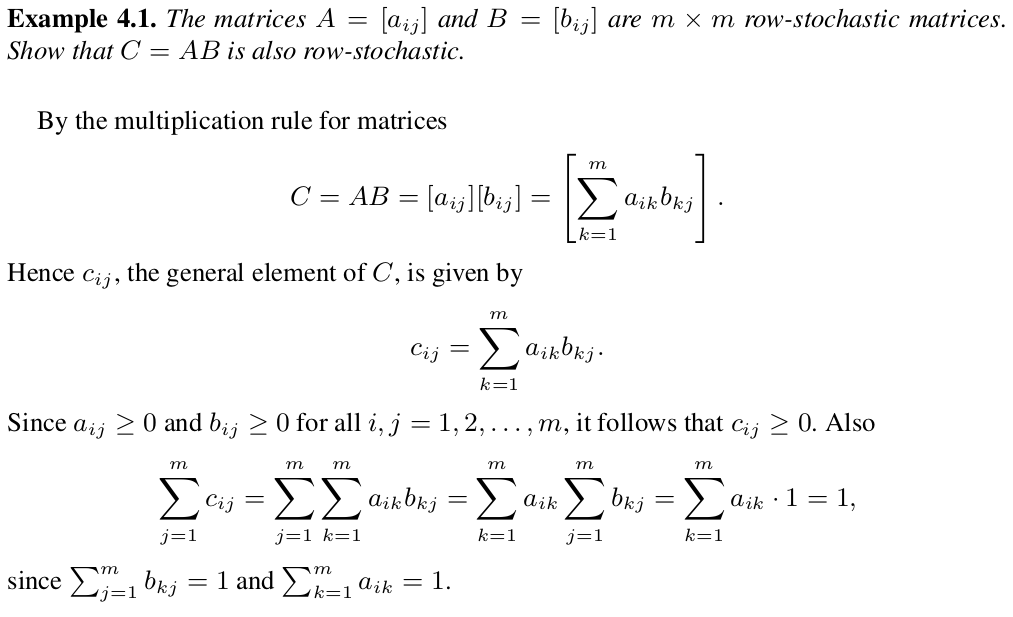
\includegraphics[scale=0.3]{im1}
\end{center}

\end{frame}
%%%%%%%%%%%%%%%%%%%%%%%%%%%%%%%%%%%%%%%%%%%%%%%%%%%%%%%%%%%%%%%%%%%%%%%%%%%%%%%%%%%%%%%%%%%%%%%%%%%%%%%%%%%%%
\begin{frame}
\frametitle{Probabilidad estacionaria o absoluta}
Otra probabilidad de interés es la del resultado $E_{j}$ después de $n$ pasos, dada una distribución de probabilidad inicial $\lbrace p_{i}^{(0)}\rbrace$.  Donde $p_{i}^{(0)}$ es la probabilidad que inicialmente el sistema ocupe el estado $E_{i}$. Seguro $\sum_{i=1}^{m}p_{i}^{0}=1$. Sea $p_{j}^{(1)}$  la probabilidad de que $E_{j}$ sea ocupado después de un paso. Por la ley de probabilidad total 
\begin{equation*}
p_{j}^{(1)}= \sum_{i=1}^{m}p_{i}^{(0)} p_{ij}
\end{equation*}
podemos expresar $p^{(0)}$ y $p^{(1)}$ esto como dos vectores 
\begin{equation*}
\textbf{p}^{(0)}= \left[ p_{1}^{(0)} p_{2}^{(0)}  \ldots p_{m}^{(0)} \right]  
\end{equation*}

\begin{equation*}
\textbf{p}^{(1)}= \left[ p_{1}^{(1)} p_{2}^{(1)}  \ldots p_{m}^{(1)} \right]  
\end{equation*}


\end{frame}
%%%%%%%%%%%%%%%%%%%%%%%%%%%%%%%%%%%%%%%%%%%%%%%%%%%%%%%%%%%%%%%%%%%%%%%%%%%%%%%%%%%%%%%%%%%%%%%%%%%%%%%%%%%%%
\begin{frame}
\frametitle{Probabilidad estacionaria o absoluta}

La expresión $p_{j}^{(1)}= \sum_{i=1}^{m}p_{i}^{(0)} p_{ij}$ puede ser representada como un producto matricial 


\begin{equation*}
\textbf{p}^{(1)}= \left[ p_{j}^{(1)} \right] = \left[ \sum_{i=1}^{m}p_{i}^{(0)} p_{ij} \right]  =\textbf{p}^{(0)}T´
\end{equation*}


\end{frame}
%%%%%%%%%%%%%%%%%%%%%%%%%%%%%%%%%%%%%%%%%%%%%%%%%%%%%%%%%%%%%%%%%%%%%%%%%%%%%%%%%%%%%%%%%%%%%%%%%%%%%%%%%%%%%
\begin{frame}
\frametitle{Probabilidad estacionaria o absoluta}

Sí $p^{(2)}$ es la distribución después de dos pasos, entonces 

\begin{equation*}
\textbf{p}^{(2)}= \textbf{p}^{(1)} T= \textbf{p}^{(0)}TT = \textbf{p}^{(0)}T^2 
\end{equation*}

por lo tanto después de n pasos de repetir el proceso tenemos 


\begin{equation*}
\textbf{p}^{(n)}= \textbf{p}^{(n-1)} T= \textbf{p}^{(0)}T^{n} 
\end{equation*}
donde

\begin{equation*}
\textbf{p}^{(n)}= \left[ p_{1}^{(n)} p_{2}^{(n)}  \ldots p_{m}^{(n)} \right]  
\end{equation*}

Más generalmente 

\begin{equation*}
\textbf{p}^{(n+r)}=\textbf{p}^{(r)}T^n 
\end{equation*}
\end{frame}
%%%%%%%%%%%%%%%%%%%%%%%%%%%%%%%%%%%%%%%%%%%%%%%%%%%%%%%%%%%%%%%%%%%%%%%%%%%%%%%%%%%%%%%%%%%%%%%%%%%%%%%%%%%%%
\begin{frame}
\frametitle{Probabilidad estacionaria o absoluta}

En $\textbf{p}^{(n)}= \left[ p_{1}^{(n)} p_{2}^{(n)}  \ldots p_{m}^{(n)} \right]  $, el término $p_{j}^{(n)}$ es la probabilidad absoluta o no condicional del resultado $E_{j}$ en el paso $n-th$ dada la distribución inicial $p^{0}$, esto es,
$P \left\lbrace  X_{n}= j \right\rbrace  = p_{j}^{(n)}$. Notese que \begin{equation*}
\sum_{j=1}^{m}{p_{j}^{(n)}}=1
\end{equation*} 
\end{frame}
%%%%%%%%%%%%%%%%%%%%%%%%%%%%%%%%%%%%%%%%%%%%%%%%%%%%%%%%%%%%%%%%%%%%%%%%%%%%%%%%%%%%%%%%%%%%%%%%%%%%%%%%%%%%%

\begin{frame}
\frametitle{Probabilidad estacionaria o absoluta}
Ejercicio. En una cadena de Markov triestado, $E_{1} ,E_{2} ,E_{3}$, cuyo inicio de la cadena es $E_{2}$ de tal manera que la $\textbf{p}^{(0)}= \left[ 0, 1, 0 \right]  $. Encuentre la probabilidad absoluta $\textbf{p}^{(3)}$ si matriz de transición es 

\begin{equation}
T =\begin{bmatrix}
1/2 & 1/4 & 1/4 \\
0 & 1/2 & 1/2  \\
3/4 & 1/4 & 0 
\end{bmatrix}
\end{equation} 
 
\end{frame}

%%%%%%%%%%%%%%%%%%%%%%%%%%%%%%%%%%%%%%%%%%%%%%%%%%%%%%%%%%%%%%%%%%%%%%%%%%%%%%%%%%%%%%%%%%%%%%%%%%%%%%%%%%%%%

\begin{frame}
\frametitle{Probabilidad de transición en el paso-n $p_{ij}^{(n)}$}
Ahora definimos $p_{ij}^{(n)}$ como la probabilidad de que la cadena esté en el estado $E_{j}$ después de $n$ pasos dado que la cadena comenzó en el estado $E_{i}$. Las probabilidades de transición del primer paso $p_{ij} = p_{ij}$ son simplemente los elementos de la matriz de transición $T$. Si tenemos la intención de encontrar una fórmula para $p^{(n)}_{ij}$. Ahora, por definición,
 \begin{equation*}
 p_{ij}^{(n)}=P(X_{n}=j \vert X_{0}=i)
 \end{equation*}
 también 
  \begin{equation*}
 p_{ij}^{(n)}=\sum_{k=1}^{m} P(X_{n}=j, X_{n-1}=k \vert X_{0}=i)
 \end{equation*}
 para $n \geq 2$ ya que la cadena debe haber pasado por uno de todos los m estados posibles en el paso $n-1$.
\end{frame}
%%%%%%%%%%%%%%%%%%%%%%%%%%%%%%%%%%%%%%%%%%%%%%%%%%%%%%%%%%%%%%%%%%%%%%%%%%%%%%%%%%%%%%%%%%%%%%%%%%%%%%%%%%%%%

\begin{frame}
\frametitle{Probabilidad de transición en el paso-n $p_{ij}^{(n)}$}
Ahora definimos $p_{ij}^{(n)}$ como la probabilidad de que la cadena esté en el estado $E_{j}$ después de $n$ pasos dado que la cadena comenzó en el estado $E_{i}$. Las probabilidades de transición del primer paso $p_{ij} = p_{ij}$ son simplemente los elementos de la matriz de transición $T$. Si tenemos la intención de encontrar una fórmula para $p^{(n)}_{ij}$. Ahora, por definición,
 \begin{equation*}
 p_{ij}^{(n)}=P(X_{n}=j \vert X_{0}=i)
 \end{equation*}
 también 
  \begin{equation*}
 p_{ij}^{(n)}=\sum_{k=1}^{m} P(X_{n}=j, X_{n-1}=k \vert X_{0}=i)
 \end{equation*}
 para $n \geq 2$ ya que la cadena debe haber pasado por uno de todos los m estados posibles en el paso $n-1$.
\end{frame}

%%%%%%%%%%%%%%%%%%%%%%%%%%%%%%%%%%%%%%%%%%%%%%%%%%%%%%%%%%%%%%%%%%%%%%%%%%%%%%%%%%%%%%%%%%%%%%%%%%%%%%%%%%%%%

\begin{frame}
\frametitle{Probabilidad de transición en el paso-n $p_{ij}^{(n)}$}
Para tres eventos cualesquiera $A,B,$ y $C$, tenemos la siguiente identidad 
\begin{equation*}
P(A \cap B \vert C) = P(A \vert B \cap C) P(B \vert C) 
\end{equation*} 
Interpretando $A$ como $X_n = j$, $B$ como $X_{n-1} = k$, and $C$ as $X_{0} = i$, queda como sigue 
\small
\begin{align*} 
p_{ij}^{(n)}& = P(A \cap B \vert C) = P(X_{n}=j, X_{n-1}=k \vert X_{0}=i) \\
& =\sum_{k=1}^{m}
(X_{n}=j\vert X_{n-1}=k,  X_{0}=i) P(X_{n-1}=k \vert X_{0}=i)\\
& =\sum_{k=1}^{m}P(X_{n}=j\vert X_{n-1}=k) P(X_{n-1}=k \vert X_{0}=i)\\
& =\sum_{k=1}^{m} p_{kj}^{(1)}p_{ik}^{n-1}
\end{align*}

\end{frame}

%%%%%%%%%%%%%%%%%%%%%%%%%%%%%%%%%%%%%%%%%%%%%%%%%%%%%%%%%%%%%%%%%%%%%%%%%%%%%%%%%%%%%%%%%%%%%%%%%%%%%%%%%%%%%

\begin{frame}
\frametitle{Probabilidad de transición en el paso-n $p_{ij}^{(n)}$}
Las ecuaciones anteriores son conocidas como las ecuaciones de  Chapman-Kolmogorov. Poniendo $n$ sucesivamente igual a $2, 3, \ldots$, encontramos que las matrices tiene estos elementos, usando la regla del producto para matrices, 
\begin{equation*}
\left[ {p_{ij}}^{(2)} \right] = \left[ \sum_{k=1}^{m} p_{kj}^{(1)}p_{kj}^{(1)} \right] =  T^2
\end{equation*} 

\begin{equation*}
\left[ {p_{ij}}^{(3)} \right] = \left[ \sum_{k=1}^{m} p_{kj}^{(2)}p_{kj}^{(1)} \right] =  T^2T=T^3
\end{equation*}

ya que ${p_{ij}}^{(2)} $ son los elementos de $T^2$ y así sucesivamente, la regla se generaliza a 
\begin{equation*}
\left[ {p_{ij}}^{(n)} \right]=T^n
\end{equation*}
\end{frame}

%%%%%%%%%%%%%%%%%%%%%%%%%%%%%%%%%%%%%%%%%%%%%%%%%%%%%%%%%%%%%%%%%%%%%%%%%%%%%%%%%%%%%%%%%%%%%%%%%%%%%%%%%%%%%

\begin{frame}
\frametitle{Ejemplo}
En una determinada región, los patrones climáticos tienen la siguiente secuencia. Un día se describe como soleado (S) si el sol brilla durante más del 50\% de las horas de luz y nublado (C) si el sol brilla durante menos del 50\% de las horas de luz. Los datos indican que si está nublado un día, es igualmente probable que esté nublado o soleado al día siguiente; si hace sol hay una probabilidad de 1/3 de que esté nublado y de 2/3 de que esté soleado al día siguiente.

\begin{enumerate}
\item Construya la matriz de transición T para este proceso.
\item Si hoy está nublado, ¿cuáles son las probabilidades de que a) esté nublado, b) soleado, dentro de tres días?
\item Calcule $T^5$ y $T^{10}$. ¿Cómo crees que $T^n$ se comporta cuando $n \rightarrow  \infty$? ¿Cómo se comporta $p^{(n)}$ cuando $n \rightarrow  \infty$? ¿Espera que el límite dependa de $p^{(0)}$?
\end{enumerate}
\end{frame}



%%%%%%%%%%%%%%%%%%%%%%%%%%%%%%%%%%%%%%%%%%%%%%%%%%%%%%%%%%%%%%%%%%%%%%%%%%%%%%%%%%%%%%%%%%%%%%%%%%%%%%%%%%%%%


\begin{frame}
\frametitle{Ejemplo}
\begin{enumerate}
\item Construya la matriz de transición T para este proceso.
\end{enumerate}

Se asume que es un proceso Markoviano. Cadena de dos estados 

\begin{center}
$E_{1}=$ (clima nublado, C) \hspace{2em} $E_{2}=$ (clima soleado, S)
\end{center} 
Matriz de transición 
\begin{columns}
\column{0.5\textwidth}
\begin{center}
\begin{tabular}{ c c c }
  & C & S \\ 
  \hline
 C & 1/2 & 1/2 \\  
 S & 1/3 & 2/3    
\end{tabular}
\end{center}
\column{0.5\textwidth}
\begin{center}

\begin{equation*}
T= \begin{bmatrix}
1/2 & 1/2 \\
1/3 & 2/3  
\end{bmatrix}
\end{equation*}

\end{center}
\end{columns}
Las probabilidades de transición actuales son

\begin{equation*}
p_{11} = 1/2, \quad p_{12} = 1/2,  \quad p_{21} = 1/3,  \quad p_{22} = 2/3
\end{equation*}



\end{frame}

%%%%%%%%%%%%%%%%%%%%%%%%%%%%%%%%%%%%%%%%%%%%%%%%%%%%%%%%%%%%%%%%%%%%%%%%%%%%%%%%%%%%%%%%%%%%%%%%%%%%%%%%%%%%%


\begin{frame}
\frametitle{Ejemplo}
\begin{enumerate}
\setcounter{enumi}{2}
\item Si hoy está nublado, ¿cuáles son las probabilidades de que a) esté nublado, b) soleado, dentro de tres días?
\end{enumerate}

\begin{equation*}
\textbf{p}^{(0)}=\left[ p_{1}^{(0)} \quad p_{2}^{(0)}\right] =\left[ 1 \quad  0 \right]  
\end{equation*}
lo que significa que hoy está nublado. Dentro de tres días
\small
\begin{align*} 
\textbf{p}^{(3)}  & = \left[ 1 \quad  0 \right] {\begin{bmatrix} 1/2 & 1/2 \\ 1/3 & 2/3   \end{bmatrix}} ^3\\
& =\left[ 1 \quad  0 \right] {\begin{bmatrix} 29/72 & 43/72 \\ 43/108 & 65/108  \end{bmatrix}} \\
& =\left[ 29/72 \quad  43/72 \right] = \left[ 0.40278 \quad  0.59722 \right]
\end{align*}
Por lo que las probabilidades son: (a) $p_{1}^{(3)}= 29/72$ y (b) $p_{2}^{(3)}=43/72$ 
\end{frame}
%%%%%%%%%%%%%%%%%%%%%%%%%%%%%%%%%%%%%%%%%%%%%%%%%%%%%%%%%%%%%%%%%%%%%%%%%%%%%%%%%%%%%%%%%%%%%%%%%%%%%%%%%%%%%


\begin{frame}
\frametitle{Cadena de Markov general bi-estado}
Considere  la siguiente matriz de transición
\begin{center}
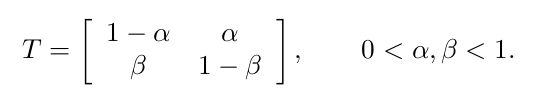
\includegraphics[scale=0.4]{im2}
\end{center}
Queremos encontrar un fórmula general para $T^{n}$. Primero encontramos los eigenvalores ($\lambda$)de $T$ con $det(T-\lambda I_{2})=0$
\begin{center}
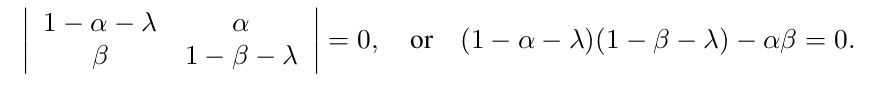
\includegraphics[scale=0.35]{im3}
\end{center}
\end{frame}
%%%%%%%%%%%%%%%%%%%%%%%%%%%%%%%%%%%%%%%%%%%%%%%%%%%%%%%%%%%%%%%%%%%%%%%%%%%%%%%%%%%%%%%%%%%%%%%%%%%%%%%%%%%%%


\begin{frame}
\frametitle{Cadena de Markov general bi-estado}
\begin{center}
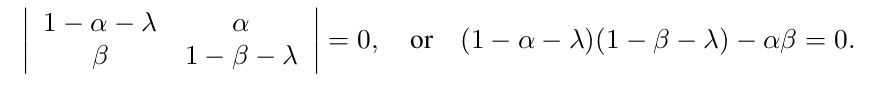
\includegraphics[scale=0.35]{im3}
\end{center}
Resolviendo
\begin{center}
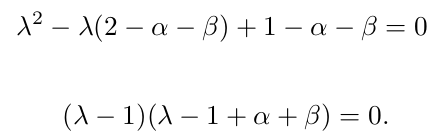
\includegraphics[scale=0.4]{im4}
\end{center}
Los eigenvalores de T son $\lambda_{1}=1$ y $\lambda_{2}= 1-\alpha-\beta =s$. Notese que las matrices estocásticas siempre va a tener un eigenvalor unitario.
\end{frame}
%%%%%%%%%%%%%%%%%%%%%%%%%%%%%%%%%%%%%%%%%%%%%%%%%%%%%%%%%%%%%%%%%%%%%%%%%%%%%%%%%%%%%%%%%%%%%%%%%%%%%%%%%%%%%


\begin{frame}
\frametitle{Cadena de Markov general bi-estado}
Los eigenvalores de T son $\lambda_{1}=1$ y $\lambda_{2}= 1-\alpha-\beta =s$. 

Encontrando los eigenvectores asociados a los eigenvalores. Sea $\textbf{r}_{1}$ es eigenvector de $\lambda_{1}$ definido por 


\begin{center}
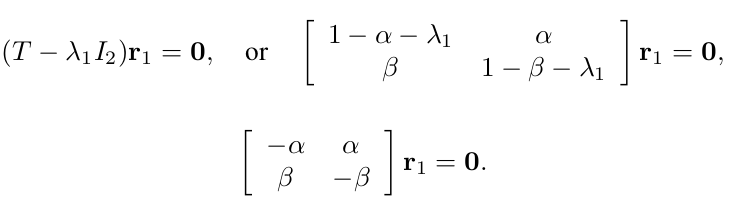
\includegraphics[scale=0.4]{im5}
\end{center}


\end{frame}
%%%%%%%%%%%%%%%%%%%%%%%%%%%%%%%%%%%%%%%%%%%%%%%%%%%%%%%%%%%%%%%%%%%%%%%%%%%%%%%%%%%%%%%%%%%%%%%%%%%%%%%%%%%%%


\begin{frame}
\frametitle{Cadena de Markov general bi-estado}

\begin{center}
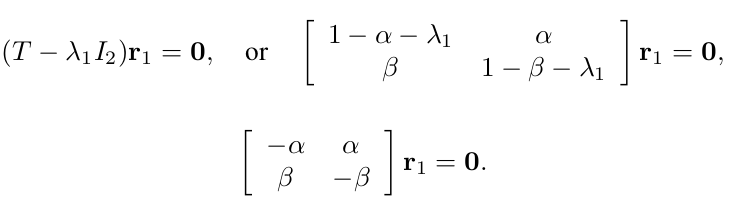
\includegraphics[scale=0.4]{im5}
\end{center}
Encontrando alguna solución no trivial a la esta ecuación 
\begin{center}
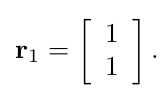
\includegraphics[scale=0.4]{im6}
\end{center}

Notese que el vector asociado a eigenvalor unitario es un vector de unos.
\end{frame}

%%%%%%%%%%%%%%%%%%%%%%%%%%%%%%%%%%%%%%%%%%%%%%%%%%%%%%%%%%%%%%%%%%%%%%%%%%%%%%%%%%%%%%%%%%%%%%%%%%%%%%%%%%%%%
\begin{frame}
\frametitle{Cadena de Markov general bi-estado}
De manera similar encontramos los eigenvectores para $\lambda_{2}= 1-\alpha-\beta =s$. 

\begin{center}
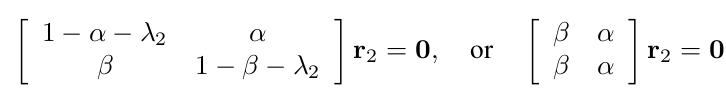
\includegraphics[scale=0.4]{im7}
\end{center}
para este caso el vector queda 
\begin{center}
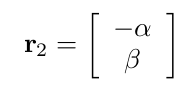
\includegraphics[scale=0.4]{im8}
\end{center}



\end{frame}
%%%%%%%%%%%%%%%%%%%%%%%%%%%%%%%%%%%%%%%%%%%%%%%%%%%%%%%%%%%%%%%%%%%%%%%%%%%%%%%%%%%%%%%%%%%%%%%%%%%%%%%%%%%%%
\begin{frame}
\frametitle{Cadena de Markov general bi-estado}
Ahora formamos la matriz C con los eigenvectores 

\begin{center}
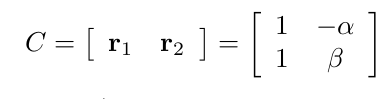
\includegraphics[scale=0.4]{im9}
\end{center}

obtenemos su inversa

\begin{center}
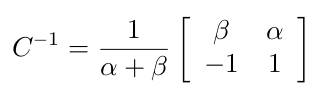
\includegraphics[scale=0.4]{im10}
\end{center}

\end{frame}
%%%%%%%%%%%%%%%%%%%%%%%%%%%%%%%%%%%%%%%%%%%%%%%%%%%%%%%%%%%%%%%%%%%%%%%%%%%%%%%%%%%%%%%%%%%%%%%%%%%%%%%%%%%%%
\begin{frame}
\frametitle{Cadena de Markov general bi-estado}
Si expandimos el producto matricial $C^{-1}TC$ tenemos 
\begin{center}
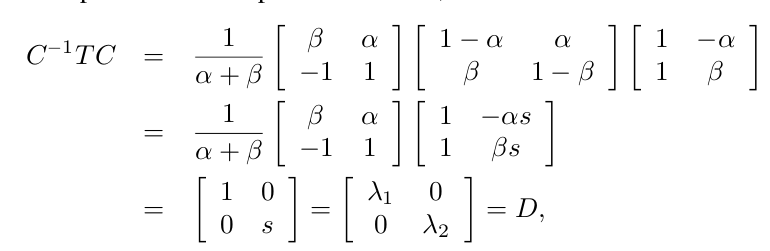
\includegraphics[scale=0.4]{im11}
\end{center}
Ahora $D$ es una matriz diagonal con los valores propios de $T$ como sus elementos diagonales: este proceso se conoce en álgebra lineal como la diagonalización de una matriz.El resultado es significativo ya que las matrices diagonales son fáciles de multiplicar.
\end{frame}
%%%%%%%%%%%%%%%%%%%%%%%%%%%%%%%%%%%%%%%%%%%%%%%%%%%%%%%%%%%%%%%%%%%%%%%%%%%%%%%%%%%%%%%%%%%%%%%%%%%%%%%%%%%%%
\begin{frame}
\frametitle{Cadena de Markov general bi-estado}
Para el caso de potencias
\begin{center}
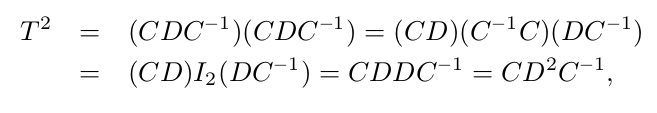
\includegraphics[scale=0.4]{im12}
\end{center}
donde
\begin{center}
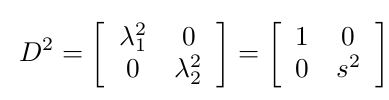
\includegraphics[scale=0.4]{im13}
\end{center}
se puede probar que 
\begin{center}
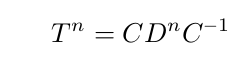
\includegraphics[scale=0.4]{im14}
\end{center}
\end{frame}
%%%%%%%%%%%%%%%%%%%%%%%%%%%%%%%%%%%%%%%%%%%%%%%%%%%%%%%%%%%%%%%%%%%%%%%%%%%%%%%%%%%%%%%%%%%%%%%%%%%%%%%%%%%%%
\begin{frame}
\frametitle{Cadena de Markov general bi-estado}
se puede probar que 
\begin{center}
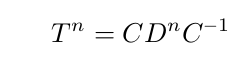
\includegraphics[scale=0.4]{im14}
\end{center}
con
\begin{center}
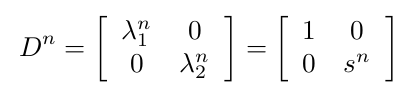
\includegraphics[scale=0.4]{im15}
\end{center}

\end{frame}
%%%%%%%%%%%%%%%%%%%%%%%%%%%%%%%%%%%%%%%%%%%%%%%%%%%%%%%%%%%%%%%%%%%%%%%%%%%%%%%%%%%%%%%%%%%%%%%%%%%%%%%%%%%%%
\begin{frame}
\frametitle{Cadena de Markov general bi-estado}
Entonces el producto de matrices queda como 

\begin{center}
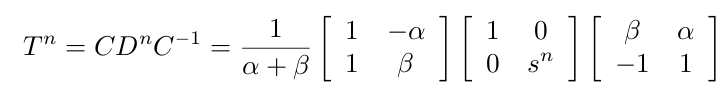
\includegraphics[scale=0.4]{im16}
\end{center}

dado que $0<\alpha,\beta < 1$, además $\vert s\vert <1$ y si $n\rightarrow \infty $ entonces $s^{n} \rightarrow 0$ por lo tanto
\begin{center}
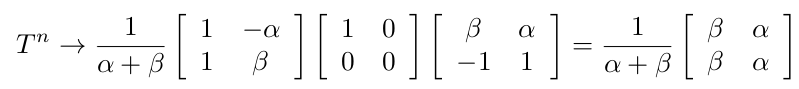
\includegraphics[scale=0.4]{im17}
\end{center}

\end{frame}
%%%%%%%%%%%%%%%%%%%%%%%%%%%%%%%%%%%%%%%%%%%%%%%%%%%%%%%%%%%%%%%%%%%%%%%%%%%%%%%%%%%%%%%%%%%%%%%%%%%%%%%%%%%%%
\begin{frame}
\frametitle{Cadena de Markov general bi-estado}
Por lo tanto para cualquier distribución de probabilidad inicial $\textbf{p}_{0}$, la distribución sobre los estados después de n pasos esta dada por 
\begin{center}
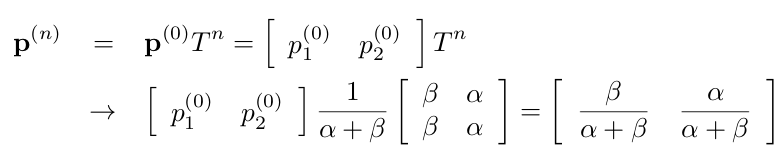
\includegraphics[scale=0.4]{im18}
\end{center}
se puede notar que conforme  $n\rightarrow \infty $  el limite es independiente de $\textbf{p}^{(0)}$. Esto es un ejemplo de una distribución invariante de la cadena de Markov, ya que es independiente de la distribución inicial. Se dice que la cadena está en equilibrio.
\end{frame}
%%%%%%%%%%%%%%%%%%%%%%%%%%%%%%%%%%%%%%%%%%%%%%%%%%%%%%%%%%%%%%%%%%%%%%%%%%%%%%%%%%%%%%%%%%%%%%%%%%%%%%%%%%%%%
\begin{frame}
\frametitle{Cadena de Markov general bi-estado}
¿Qué sucede con el limite si $\alpha=\beta=1$? ¿y qué sucede si $\alpha = 1, 0 < \beta < 1$ or $0 < \alpha < 1$, $\beta = 1$?.
tenga presente 
\begin{equation*}
s=1-\alpha-\beta
\end{equation*}

\begin{center}
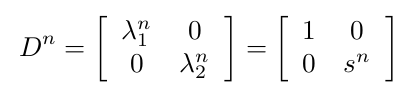
\includegraphics[scale=0.4]{im15}
\end{center}
\begin{center}
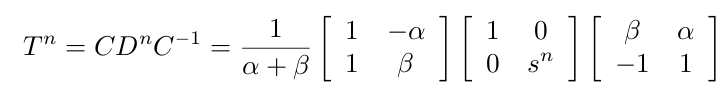
\includegraphics[scale=0.4]{im16}
\end{center}
\end{frame}

%%%%%%%%%%%%%%%%%%%%%%%%%%%%%%%%%%%%%%%%%%%%%%%%%%%%%%%%%%%%%%%%%%%%%%%%%%%%%%%%%%%%%%%%%%%%%%%%%%%%%%%%%%%%%
\begin{frame}
\frametitle{Cadena de Markov general bi-estado}
El método derivado para la cadena de dos estados en la sección anterior se puede generalizar a cadenas de m-estados.Sea $T$ una matriz estocástica $m x m$, en otras palabras, una posible matriz de transición. Los eigenvalores de T están dados por
\begin{center}
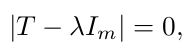
\includegraphics[scale=0.4]{im19}
\end{center}
donde $I_{m}$ es la matriz identidad de orden $m$. Suponga que los valores propios son distintos y se denotan por $\lambda_{1}, \lambda_{2},\ldots ,\lambda_{m}$.
\end{frame}
%%%%%%%%%%%%%%%%%%%%%%%%%%%%%%%%%%%%%%%%%%%%%%%%%%%%%%%%%%%%%%%%%%%%%%%%%%%%%%%%%%%%%%%%%%%%%%%%%%%%%%%%%%%%%
\begin{frame}
\frametitle{Cadena de Markov general bi-estado}
Nuevamente note que la matriz estocástica $T$ siempre tiene un eigenvalor unitario, digamos $\lambda_{1}=1$ con un eigenvector unitario

\begin{center}
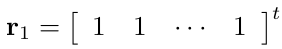
\includegraphics[scale=0.4]{im20}
\end{center}
Todos los vectores tiene que satisfacer 
\begin{center}
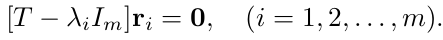
\includegraphics[scale=0.4]{im21}
\end{center}
la matriz C quedaría como 
\begin{center}
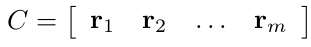
\includegraphics[scale=0.4]{im22}
\end{center}
\end{frame}
%%%%%%%%%%%%%%%%%%%%%%%%%%%%%%%%%%%%%%%%%%%%%%%%%%%%%%%%%%%%%%%%%%%%%%%%%%%%%%%%%%%%%%%%%%%%%%%%%%%%%%%%%%%%%
\begin{frame}
\frametitle{Cadena de Markov general bi-estado}
La matriz C nos sirve para diagonalizar la matriz T, quedando como 


\begin{center}
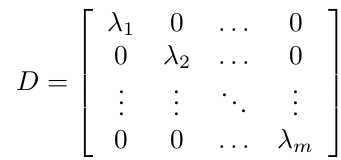
\includegraphics[scale=0.3]{im23}
\end{center}
la cual es útil para estimar la potencia n
\begin{center}
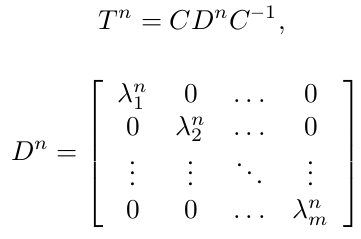
\includegraphics[scale=0.3]{im24}
\end{center}

\end{frame}
%%%%%%%%%%%%%%%%%%%%%%%%%%%%%%%%%%%%%%%%%%%%%%%%%%%%%%%%%%%%%%%%%%%%%%%%%%%%%%%%%%%%%%%%%%%%%%%%%%%%%%%%%%%%%
\begin{frame}
\frametitle{Cadena de Markov general bi-estado}
\textbf{Ejercicio 1}

Encuentre los eigenvalores y eigenvectores de la matriz estocástica 

\begin{center}
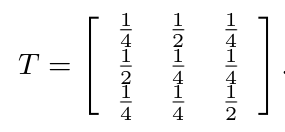
\includegraphics[scale=0.3]{im25}
\end{center}

Encuentre una fórmula para $T^{n}$, y encuentre el $lim_{n\rightarrow \infty}$ $T^{n}$.
\end{frame}

%%%%%%%%%%%%%%%%%%%%%%%%%%%%%%%%%%%%%%%%%%%%%%%%%%%%%%%%%%%%%%%%%%%%%%%%%%%%%%%%%%%%%%%%%%%%%%%%%%%%%%%%%%%%%

\begin{frame}
\frametitle{Cadena de Markov general bi-estado}
\textbf{Ejercicio 2}


Los estados absorbentes son reconocibles en las cadenas de Markov por un valor 1 en un elemento diagonal de la matriz de transición. Dado que tales matrices son estocásticas, todos los demás elementos de la misma fila deben ser cero.

\begin{center}
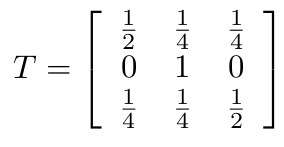
\includegraphics[scale=0.3]{im26}
\end{center}
Dibuje el grafo y encuentre una fórmula para $T^{n}$, y $lim_{n\rightarrow \infty}$ $T^{n}$.
\end{frame}
%%%%%%%%%%%%%%%%%%%%%%%%%%%%%%%%%%%%%%%%%%%%%%%%%%%%%%%%%%%%%%%%%%%%%%%%%%%%%%%%%%%%%%%%%%%%%%%%%%%%%%%%%%%%%

\begin{frame}
\frametitle{Cadena de Markov general bi-estado}
\textbf{Ejercicio 3}


Un modelo enfermedad-muerte. Un posible modelo simple enfermedad-muerte se puede representar mediante una cadena de Markov de cuatro estados en la que $E_{1}$ es un estado en el que un individuo está libre de una enfermedad particular, $E_{2}$ es un estado en el que el individuo tiene la enfermedad, y $E_3$ y $E_4$ son
respectivamente estados de muerte que surgen como consecuencia de la enfermedad o por otras causas. Durante algún intervalo de tiempo apropiado (quizás un ciclo anual), asignamos probabilidades a la transición entre los estados. Supongamos que la matriz de transición es (en el orden de los estados)

\begin{center}
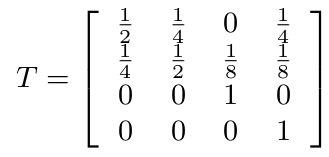
\includegraphics[scale=0.3]{im27}
\end{center}

\end{frame}
%%%%%%%%%%%%%%%%%%%%%%%%%%%%%%%%%%%%%%%%%%%%%%%%%%%%%%%%%%%%%%%%%%%%%%%%%%%%%%%%%%%%%%%%%%%%%%%%%%%%%%%%%%%%%

\begin{frame}
\frametitle{Cadena de Markov general bi-estado}
\textbf{Ejercicio 3}


Dibuje la cadena. Encuentre las probabilidades de que una persona muera finalmente después de una gran cantidad de transiciones de la enfermedad, dado que inicialmente no la padeció.

\end{frame}
%%%%%%%%%%%%%%%%%%%%%%%%%%%%%%%%%%%%%%%%%%%%%%%%%%%%%%%%%%%%%%%%%%%%%%%%%%%%%%%%%%%%%%%%%%%%%%%%%%%%%%%%%%%%%

\begin{frame}
\frametitle{Cadena de Markov general bi-estado}
\textbf{Ejercicio 4}


En el problema de la ruina de un jugador, suponga que $p$ es la probabilidad de que el jugador gane en cada jugada, y que $a = 5$ y que la apuesta inicial del jugador es $k = 3$ unidades. ¿Cuál es la probabilidad de que el jugador realmente gane en la cuarta jugada?

\end{frame}
%%%%%%%%%%%%%%%%%%%%%%%%%%%%%%%%%%%%%%%%%%%%%%%%%%%%%%%%%%%%%%%%%%%%%%%%%%%%%%%%%%%%%%%%%%%%%%%%%%%%%%%%%%%%%

\begin{frame}
\frametitle{Clasificación de estados}
\begin{block}{Estado absorbente}
En el estado absorbente una vez ingresado, no hay escapatoria. Un estado absorbente $E_i$ se caracteriza por las probabilidades

\begin{center}
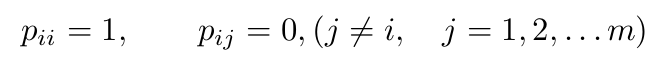
\includegraphics[scale=0.4]{im28}
\end{center}
en el $i$-th renglón de  $T$
\end{block}

\end{frame}
%%%%%%%%%%%%%%%%%%%%%%%%%%%%%%%%%%%%%%%%%%%%%%%%%%%%%%%%%%%%%%%%%%%%%%%%%%%%%%%%%%%%%%%%%%%%%%%%%%%%%%%%%%%%%

\begin{frame}
\frametitle{Clasificación de estados}
\begin{block}{Estado periódico}
La probabilidad de un retorno a $E_{i}$ en el paso $n$ es $p_{ii}^{(n)}$ . Sea $t$ un entero mayor a 1. Supongamos 

\begin{center}
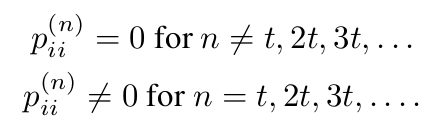
\includegraphics[scale=0.4]{im29}
\end{center}
en este caso el estado $E_i$ es periódico con periodo $t$. Si, para un estado, no existe tal $t$ con esta propiedad, entonces el estado se describe como aperiódico.
\end{block}

\end{frame}
%%%%%%%%%%%%%%%%%%%%%%%%%%%%%%%%%%%%%%%%%%%%%%%%%%%%%%%%%%%%%%%%%%%%%%%%%%%%%%%%%%%%%%%%%%%%%%%%%%%%%%%%%%%%%

\begin{frame}
\frametitle{Clasificación de estados}
\begin{block}{Regla general para estados periódico}
sea

\begin{center}
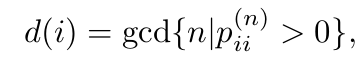
\includegraphics[scale=0.4]{im30}
\end{center}

el máximo común divisor (greatest common divisor) del conjunto de enteros $n$ para los cuales $p^{(n)}_{ii}> 0$. Entonces se dice que el estado $E_{i}$ es periódico si $d(i)> 1$ y aperiódico si $d (i) = 1$.
\end{block}

\end{frame}
%%%%%%%%%%%%%%%%%%%%%%%%%%%%%%%%%%%%%%%%%%%%%%%%%%%%%%%%%%%%%%%%%%%%%%%%%%%%%%%%%%%%%%%%%%%%%%%%%%%%%%%%%%%%%

\begin{frame}
\frametitle{Clasificación de estados}
Ejemplo de estados periódicos.

Una cadena de Markov de cuatro estados tiene la matriz de transición 
\begin{columns}
\column{0.4\textwidth}
\begin{center}
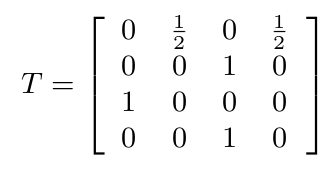
\includegraphics[scale=0.3]{im31}
\end{center}
\column{0.6\textwidth}
\begin{center}
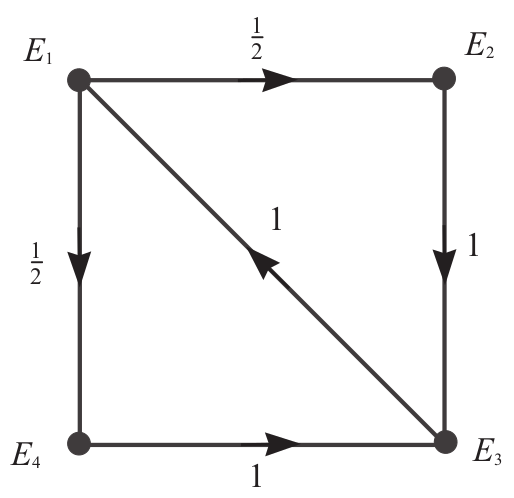
\includegraphics[scale=0.2]{im32}
\end{center}
\end{columns}

se observa que todos los estados tienen un período 3. Por ejemplo, si la cadena comienza en $E_{1}$, los retornos a $E_1$ posibles en los pasos en los pasos $3, 6, 9,\ldots$ ya sea a través de $1E_2$ o $E_3$.

\end{frame}
%%%%%%%%%%%%%%%%%%%%%%%%%%%%%%%%%%%%%%%%%%%%%%%%%%%%%%%%%%%%%%%%%%%%%%%%%%%%%%%%%%%%%%%%%%%%%%%%%%%%%%%%%%%%%

\begin{frame}
\frametitle{Clasificación de estados}
\begin{block}{Estado persistente - recurrente}
Sea $f^{(n)}_{j}$ la probabilidad de que el primer regreso a $E_{j}$ ocurra en el n-ésimo paso. Esta probabilidad no es la misma que $p^{(n)}_{jj}$, que es la probabilidad de que se produzca un retorno en el n-ésimo paso, e incluye los posibles retorno en los pasos $1, 2, 3,\ldots, n - 1$ también. Esto es 

\begin{center}
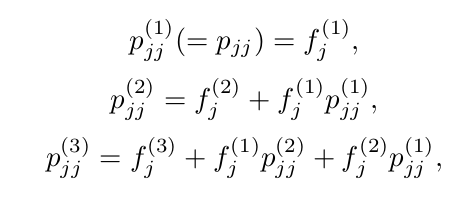
\includegraphics[scale=0.4]{im33}
\end{center}


\end{block}


\end{frame}
%%%%%%%%%%%%%%%%%%%%%%%%%%%%%%%%%%%%%%%%%%%%%%%%%%%%%%%%%%%%%%%%%%%%%%%%%%%%%%%%%%%%%%%%%%%%%%%%%%%%%%%%%%%%%

\begin{frame}
\frametitle{Clasificación de estados}
\begin{block}{Estado persistente -  recurrente}

en general
\begin{center}
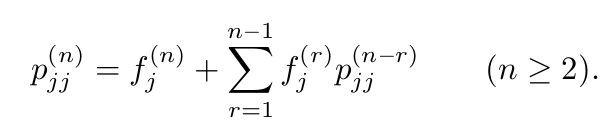
\includegraphics[scale=0.35]{im34}
\end{center}
De las ecuaciones anteriores se puede despejar $f_{j}^{(n)}$ 
\begin{center}
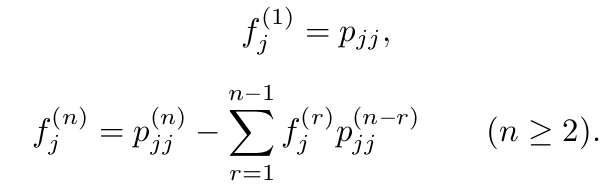
\includegraphics[scale=0.35]{im35}
\end{center}
\end{block}


\end{frame}
%%%%%%%%%%%%%%%%%%%%%%%%%%%%%%%%%%%%%%%%%%%%%%%%%%%%%%%%%%%%%%%%%%%%%%%%%%%%%%%%%%%%%%%%%%%%%%%%%%%%%%%%%%%%%

\begin{frame}
\frametitle{Clasificación de estados}

\begin{block}{Estado persistente - recurrente}
La probabilidad de que una cadena regrese en algún paso al estado $E_j$ es
\begin{center}
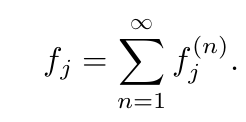
\includegraphics[scale=0.35]{im36}
\end{center}

Si $f_{j} = 1$, entonces un retorno a $E_{j}$ es seguro, y $E_{j}$ se llama \textbf{estado persistente}.
\end{block}


\end{frame}
%%%%%%%%%%%%%%%%%%%%%%%%%%%%%%%%%%%%%%%%%%%%%%%%%%%%%%%%%%%%%%%%%%%%%%%%%%%%%%%%%%%%%%%%%%%%%%%%%%%%%%%%%%%%%
\begin{frame}
\frametitle{Clasificación de estados}
Ejemplo. Estado persistente - recurrente
Una cadena de Markov de tres estados tiene la matriz de transición
\begin{center}
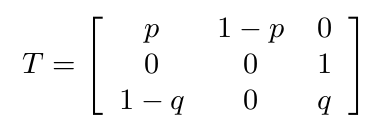
\includegraphics[scale=0.35]{im37}
\end{center}
donde $0 <p <1, 0 <q <1$. Demuestre que el estado $E_1$ es persistente.
\end{frame}
%%%%%%%%%%%%%%%%%%%%%%%%%%%%%%%%%%%%%%%%%%%%%%%%%%%%%%%%%%%%%%%%%%%%%%%%%%%%%%%%%%%%%%%%%%%%%%%%%%%%%%%%%%%%%
\begin{frame}
\frametitle{Clasificación de estados}
Diagrama de transición

\begin{center}
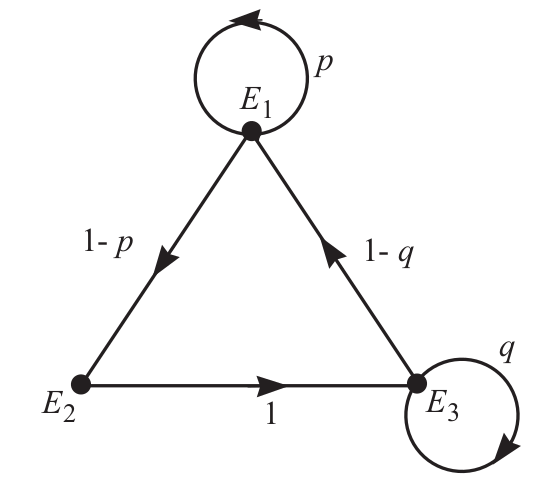
\includegraphics[scale=0.35]{im38}
\end{center}
\end{frame}

%%%%%%%%%%%%%%%%%%%%%%%%%%%%%%%%%%%%%%%%%%%%%%%%%%%%%%%%%%%%%%%%%%%%%%%%%%%%%%%%%%%%%%%%%%%%%%%%%%%%%%%%%%%%%
\begin{frame}
\frametitle{Clasificación de estados}
Si una secuencia comienza en $E_1$, entonces se puede ver que primero se pueden volver de $E_1$ a $E_1$ en cada paso excepto para $n = 2$, ya que después de dos pasos la cadena debe estar en el estado $E_3$. Entonces
\begin{center}
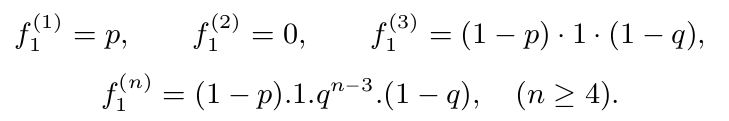
\includegraphics[scale=0.35]{im39}
\end{center}
El último resultado para $f_ {1} ^ {(n)}$ para $n \geq 4$ se deriva de la siguiente secuencia de transiciones:

\begin{center}
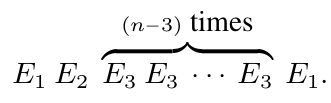
\includegraphics[scale=0.35]{im40}
\end{center}
\end{frame}

%%%%%%%%%%%%%%%%%%%%%%%%%%%%%%%%%%%%%%%%%%%%%%%%%%%%%%%%%%%%%%%%%%%%%%%%%%%%%%%%%%%%%%%%%%%%%%%%%%%%%%%%%%%%%
\begin{frame}
\frametitle{Clasificación de estados}
La probabilidad $f_{1}$ de que el sistema regrese al menos una vez a $E_{1}$ es

\begin{center}
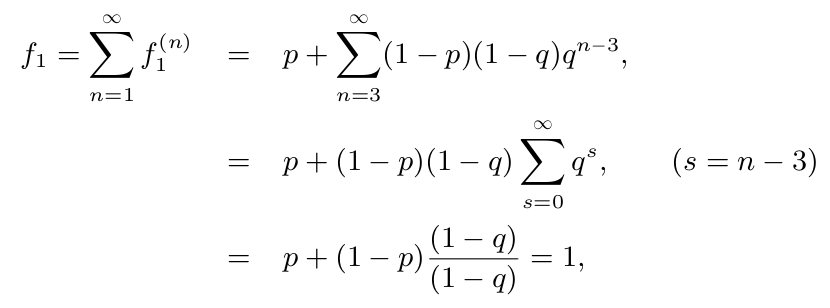
\includegraphics[scale=0.35]{im41}
\end{center}

Por tanto, $f_{1} = 1$, y en consecuencia el estado $E_1$ es persistente.

\end{frame}
%%%%%%%%%%%%%%%%%%%%%%%%%%%%%%%%%%%%%%%%%%%%%%%%%%%%%%%%%%%%%%%%%%%%%%%%%%%%%%%%%%%%%%%%%%%%%%%%%%%%%%%%%%%%%
\begin{frame}
\frametitle{Clasificación de estados}

\begin{block}{número de recurrencias promedio}
El número de recurrencias promedio $\mu_{j}$ de un estado persistente $E_{j}$, del cual $\sum_{n=1}^{\infty} f_{j}^{(n)}=1$ esta dado por 

\begin{center}
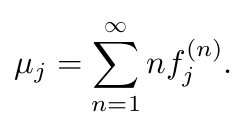
\includegraphics[scale=0.35]{im42}
\end{center}

\end{block}

\end{frame}
%%%%%%%%%%%%%%%%%%%%%%%%%%%%%%%%%%%%%%%%%%%%%%%%%%%%%%%%%%%%%%%%%%%%%%%%%%%%%%%%%%%%%%%%%%%%%%%%%%%%%%%%%%%%%
\begin{frame}
\frametitle{Clasificación de estados}
Del ejemplo anterior, el estado persistente $E_{1}$, el promedio de veces recurrentes esta dado por 


\begin{center}
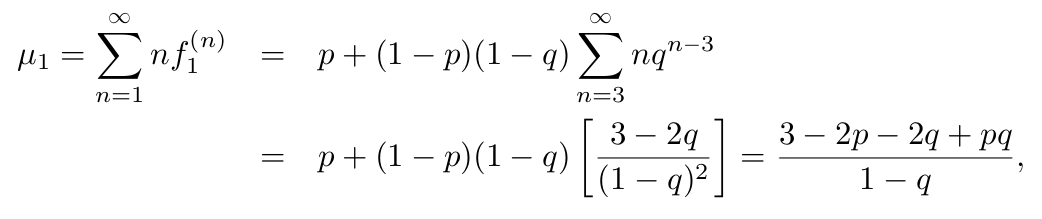
\includegraphics[scale=0.3]{im43}
\end{center}
que es finito. Para algunas cadenas, el numero medio de recurrencia puede ser infinito. Se dice que un estado persistente $E_j$ es nulo si $\mu_j = \infty$, y no nulo si $\mu_j < \infty$. 
\end{frame}
%%%%%%%%%%%%%%%%%%%%%%%%%%%%%%%%%%%%%%%%%%%%%%%%%%%%%%%%%%%%%%%%%%%%%%%%%%%%%%%%%%%%%%%%%%%%%%%%%%%%%%%%%%%%%

\begin{frame}
\frametitle{Clasificación de estados}

\begin{block}{Estado transitorio}
Para un estado persistente, la probabilidad de un primer retorno en algún paso en el futuro es cierta. Para algunos estados,
\begin{center}
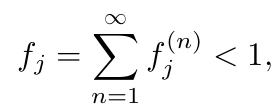
\includegraphics[scale=0.4]{im44}
\end{center}

lo que significa que la probabilidad de un primer retorno no es segura. Estos estados se describen como \textbf{transitorios}.
\end{block}

\end{frame}
%%%%%%%%%%%%%%%%%%%%%%%%%%%%%%%%%%%%%%%%%%%%%%%%%%%%%%%%%%%%%%%%%%%%%%%%%%%%%%%%%%%%%%%%%%%%%%%%%%%%%%%%%%%%%

\begin{frame}
\frametitle{Clasificación de estados}
Ejercicio. Una cadena de Markov de cuatro estados tiene la matriz de transición
 
\begin{center}
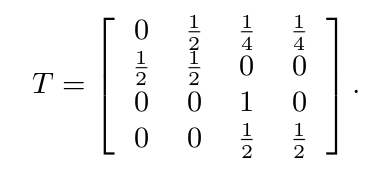
\includegraphics[scale=0.4]{im45}
\end{center}

demuestre que el estado $E_{1}$ es transitorio.


\end{frame}
%%%%%%%%%%%%%%%%%%%%%%%%%%%%%%%%%%%%%%%%%%%%%%%%%%%%%%%%%%%%%%%%%%%%%%%%%%%%%%%%%%%%%%%%%%%%%%%%%%%%%%%%%%%%%

\begin{frame}
\frametitle{Clasificación de estados}

\begin{block}{Estado ergódico}
El estado que es persistente, no nulo y aperiódico es llamado ergódico. Los estados ergódicos son importantes en la clasificación de cadenas y en la existencia de distribuciones de probabilidad limitantes.

\end{block}

\end{frame}

%%%%%%%%%%%%%%%%%%%%%%%%%%%%%%%%%%%%%%%%%%%%%%%%%%%%%%%%%%%%%%%%%%%%%%%%%%%%%%%%%%%%%%%%%%%%%%%%%%%%%%%%%%%%%

\end {document}



                                                  






